\begin{activity}\label{A:0.5.2}
    Figure \ref{fig:0.5.A1} gives us the voltage produced by an electrical circuit as a function of time.
    \begin{figure}[ht!]
    \begin{center}
%         \begin{tikzpicture}
%             \begin{axis}[axis lines=center, xmin=0, xmax=0.05, ymin=-15, ymax=55, grid,
%                     domain=0:0.05, xlabel={time (sec)}, ylabel={volts},
%                     xtick={0.005,0.01,0.015,0.02,0.025,0.03,0.035,0.04,0.045,0.05},
%                     xticklabels={0.005,0.01,0.015,0.02,0.025,0.03,0.035,0.04,0.045,0.05},
%                 ytick={-10,10,20,30,40,50}, xscale=2]
%                 \addplot[smooth, very thick, blue, samples=100]
%                 {30*sin(deg(2*pi/0.017*(x-0.008)))+20};
%             \end{axis}
%         \end{tikzpicture}
        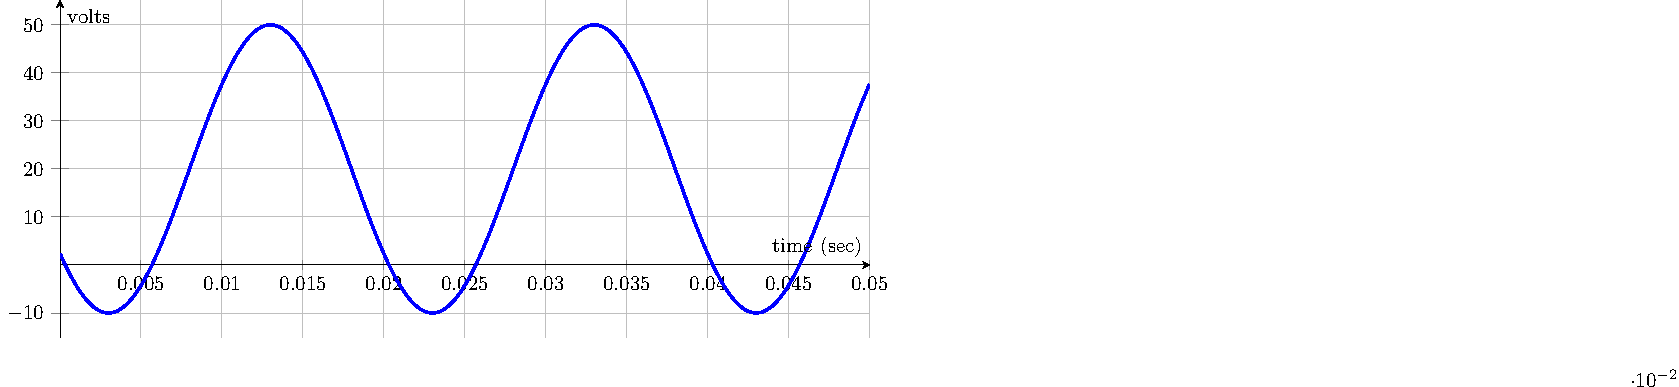
\includegraphics[trim=0cm 0cm 12cm 0cm, clip, width=0.9\columnwidth]{figures/0-5-fig9.pdf}
    \end{center}
    \caption{Voltage as a function of time.}
    \label{fig:0.5.A1}
\end{figure}
% \resizebox{5in}{!}{\includegraphics{0-5-TrigonometricFunctions5.jpg}}


\ba
\item What is the amplitude of the oscillations?  % 30 volts
\item What is the period of the oscillations? % about 0.017 seconds
\item What is the average value of the voltage?  % 20 volts
\item What is the shift along the $t$ axis, $t_0$?  % about 0.008 seconds
\item What is a formula for this function?  %  V(t) = 30 \sin( 2\pi / 0.017 ( t - 0.008) ) + 20
\ea

\end{activity}
\begin{smallhint}
    \ba
        \item measure the amplitude at half the maximum minus the minimum.
        \item measure the period from peak to peak or from trough to trough.
        \item the average value comes from the $y$ values.
        \item find the middle of the voltage values.
        \item be sure to get the shift correct.  
        \item There are infinitely many answers to this
            problem!
    \ea
\end{smallhint}
\begin{bighint}
    \ba
        \item measure the amplitude at half the maximum minus the minimum.
        \item measure the period from peak to peak or from trough to trough.
        \item the average value comes from the $y$ values.
        \item find the middle of the voltage values.
        \item be sure to get the shift correct.  
        \item There are infinitely many answers to this
            problem!
    \ea
\end{bighint}
\begin{activitySolution}
   \ba
    \item The amplitude is $A = \frac{1}{2}(50-(-10)) = 30$.
    \item The period is the distance from peak to peak.  In this case there is a peak at
        approximately $t=0.0125$ seconds and $t = 0.0325$ seconds.  Hence, the period is
        $0.02$ seconds.
    \item The average value of the voltage is 20.
    \item The simplest shift is probably to the first peak at $t = 0.0125$ seconds.
    \item $V(t) = 30 \cos\left( \frac{2\pi}{0.02} \left( t - 0.0125 \right) \right) + 20$.
   \ea
\end{activitySolution}

\aftera
